\subsection{Project2-Circle }
The endeffector needs to move in a circular anticlockwise motion as the z-axis of the simulator frame is pointing out of the scheme in Figure \ref{fig:TaskPuma}. Therefore the position trajectory of the end effector can be calculated by the following formula:
\begin{equation}
 x_d(t) = x_c + r cos(\dot{\beta} t) 
\end{equation}

\begin{equation}
     y_d(t) = y_c + r sin( \dot{\beta} t)  
\end{equation}
\newline

With the center point, the velocity and the radius defined as followed:

\begin{equation}
    x_{center}=(x_c, y_c)=(0.8m, 0.35m) 
\end{equation}
\begin{equation}
    r=0.2m
\end{equation}
\begin{equation}
    \dot{\beta}=\frac{2\pi}{5s}
\end{equation}

The desired velocity trajectory of the end effector can be consequently defined as: \\
\begin{equation}
    \dot{x}_d(t) =\frac{x(t)}{dt}= -\dot{\beta} r sin( \dot{\beta} t) 
    \label{eq:xcv}
\end{equation}
\begin{equation}
    \dot{y}_d(t) =\frac{y(t)}{dt}=  \dot{\beta} r cos( \dot{\beta} t) 
    \label{eq:ycv}
\end{equation}
\newline


The controller must keep the position of the end effector as close to the desired trajectory as possible while keeping the angle of the end effector upright. The control law to accomplish this can therefore be defined as: 

\begin{equation}
    F=\begin{pmatrix} 
  F_x \\
  F_y\\
  F_\alpha\end{pmatrix}
\end{equation}

\begin{equation}
    F_x(t)=-k_{p1}\cdot(x(t)-x_d(t)) - k_{v1}\cdot(\dot{x}(t) - \dot{x}_d(t))
\end{equation}

\begin{equation}
    F_y(t)=-k_{p1}\cdot(y(t)-y_d(t)) - k_{v1}\cdot(\dot{y}(t) - \dot{y}_d(t))
\end{equation}

\begin{equation}
    F_\alpha(t)=-k_{p1}\cdot(\alpha(t)-0) - k_{v1}\cdot(\dot{\alpha}(t) - 0)
\end{equation}

The torque that needs to be applied to the joints to control the trajectory was given in the lecture and is defined as.

\begin{equation}
    \tau= J^TF(t)
\end{equation}


In the following $\tau$, $x$, $x_d$ and $e$ are plotted for the tuned gains first (see Figures \ref{fig:CircTunedXXD}, \ref{fig:CircTunedq123}, \ref{fig:CircTunedtau}, \ref{fig:CircTunederror}, \ref{fig:CircTunedXYPLANE}). Later on for comparison lower and higher gains results can be seen (see Figures \ref{fig:LargeKpCirc}, \ref{fig:SmallKpCirc}, \ref{fig:TauComparison}). 

\begin{figure} [H]
   \begin{center}
        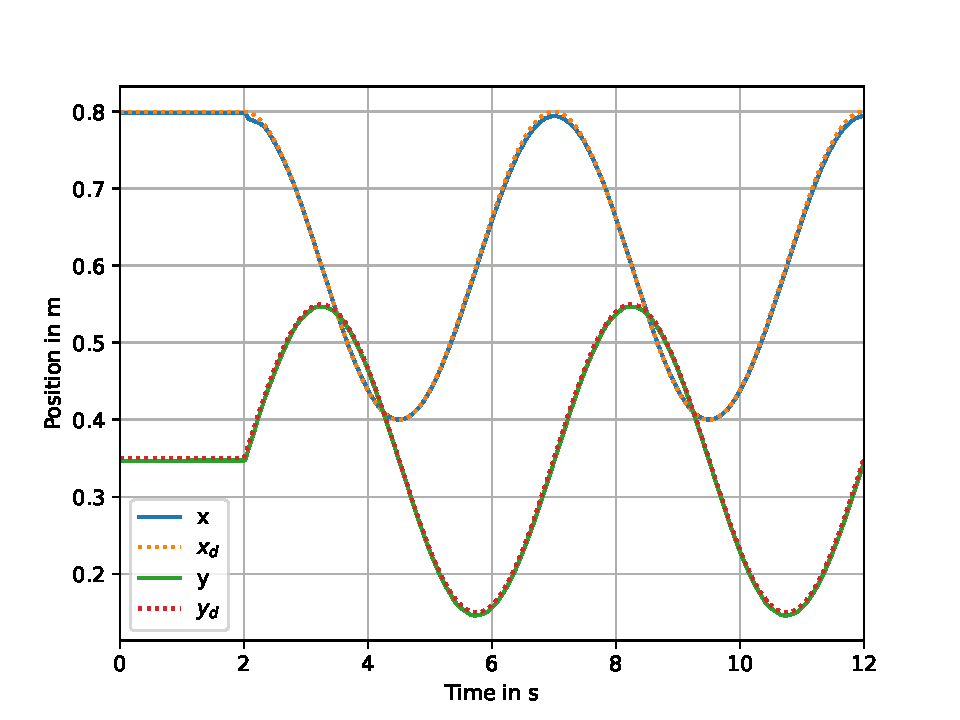
\includegraphics[width=0.7\textwidth]{SRC/CircleTraj_XandXd.pdf}
   \end{center}
  \caption{Desired and reached trajectory of proj2 control with tuned gains $k_{p1}$=26400, $k_{p2}$=22400, $k_{p2}$=1700, $k_{v1}$=140, $k_{v2}$=80, $k_{v3}$=80.}
  \label{fig:CircTunedXXD}
\end{figure}

\begin{figure} [H]
   \begin{center}
        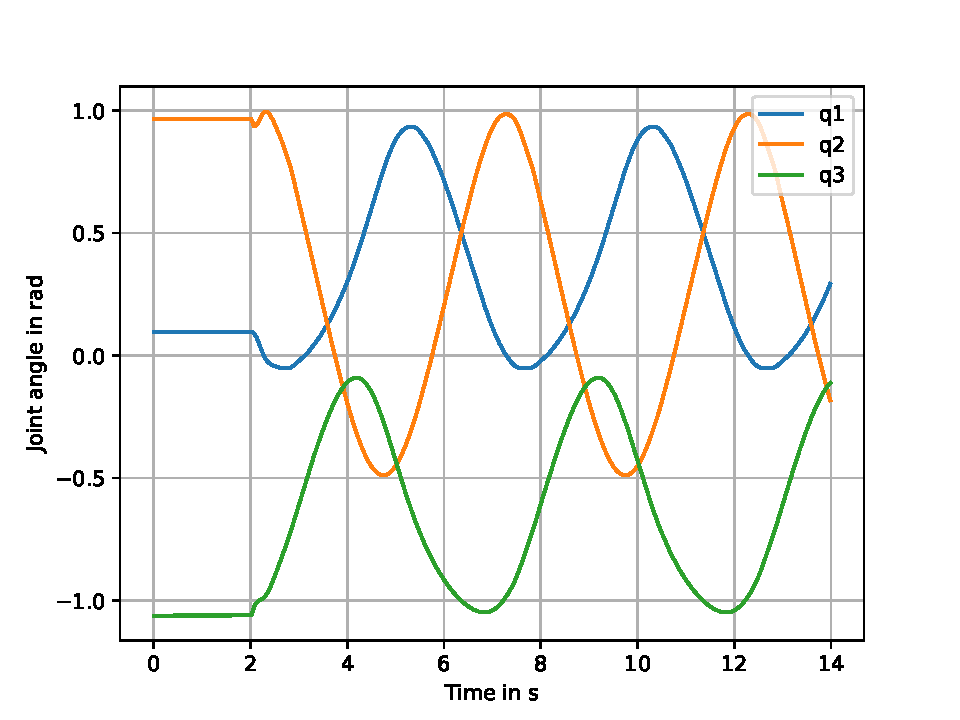
\includegraphics[width=0.7\textwidth]{SRC/CircleTraj_q1q2q3.pdf}
   \end{center}
  \caption{Joint angles during proj2 control with tuned gains $k_{p1}$=26400, $k_{p2}$=22400, $k_{p2}$=1700, $k_{v1}$=140, $k_{v2}$=80, $k_{v3}$=80.}
  \label{fig:CircTunedq123}
\end{figure}


\begin{figure} [H]
   \begin{center}
        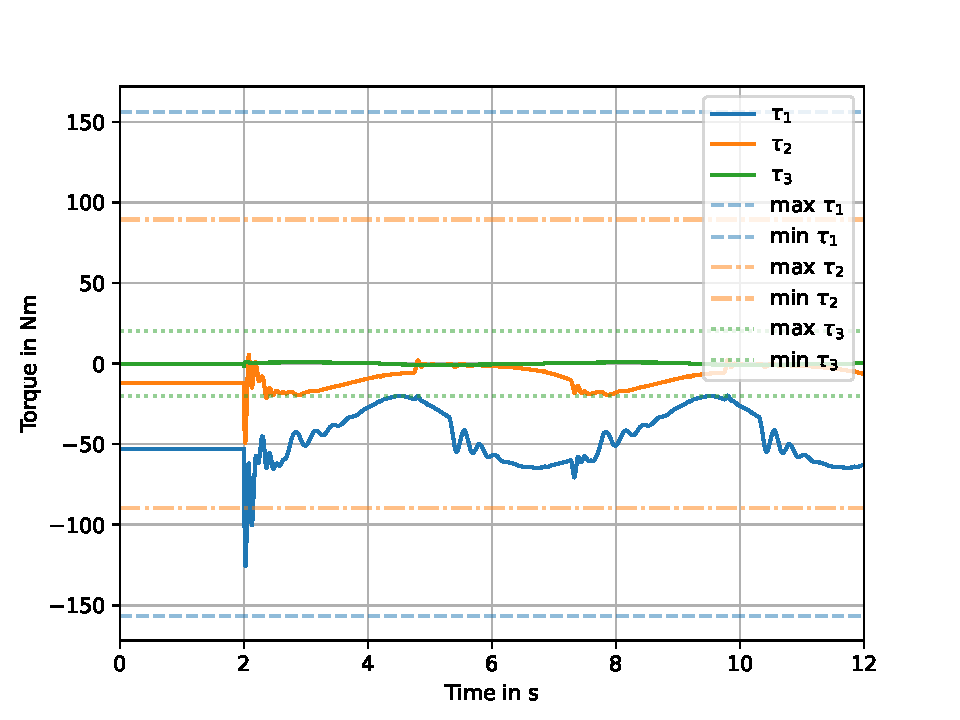
\includegraphics[width=0.7\textwidth]{SRC/CircleTraj_tau.pdf}
   \end{center}
  \caption{Joint torques during proj2 control with tuned gains $k_{p1}$=26400, $k_{p2}$=22400, $k_{p2}$=1700, $k_{v1}$=140, $k_{v2}$=80, $k_{v3}$=80.}
  \label{fig:CircTunedtau}
\end{figure}

\begin{figure} [H]
   \begin{center}
        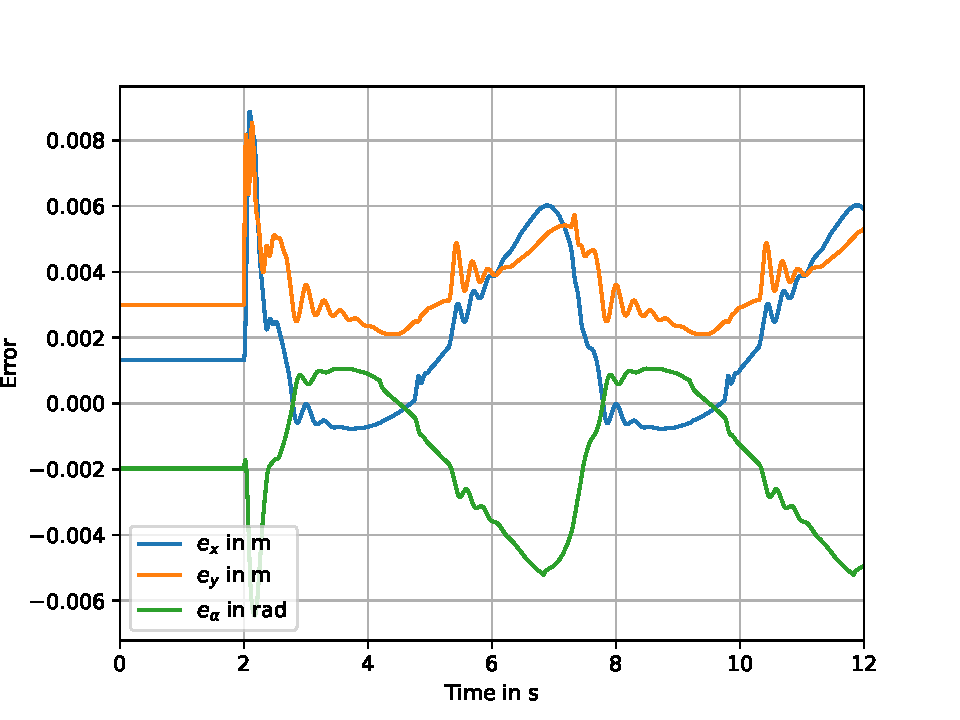
\includegraphics[width=0.7\textwidth]{SRC/CircleTraj_exeyea.pdf}
   \end{center}
  \caption{Position error during proj2 control with tuned gains $k_{p1}$=26400, $k_{p2}$=22400, $k_{p2}$=1700, $k_{v1}$=140, $k_{v2}$=80, $k_{v3}$=80.}
  \label{fig:CircTunederror}
\end{figure}


\begin{figure} [H]
   \begin{center}
        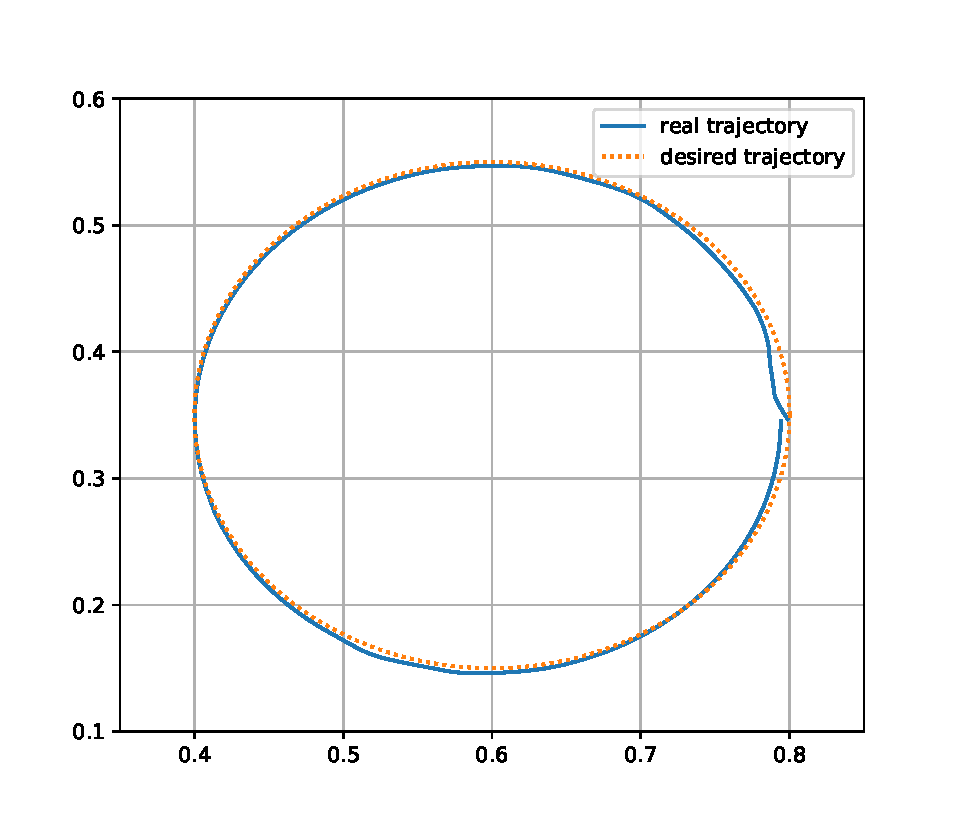
\includegraphics[width=0.7\textwidth]{SRC/CircleTraj_X_Y.pdf}
   \end{center}
  \caption{X-Y Plane trajectory during proj2 control with tuned gains $k_{p1}$=26400, $k_{p2}$=22400, $k_{p2}$=1700, $k_{v1}$=140, $k_{v2}$=80, $k_{v3}$=80.}
  \label{fig:CircTunedXYPLANE}
\end{figure}

The gains $k_{pi}$ were limited by the allowed max torque. At the beginning, where the end effector is not moving at the starting position and then should start to move is the position where maximum torques need to be applied. Therefore the gains for the tuned proj2 control were chosen so that such max torque is not exceeded. As one can see in the following figures, lower gain sets increase the error between x and $x_d$ (y-$y_d$ and $\alpha$ and $\alpha_d$). Besides that, the controller is not fast enough to follow the trajectory, so it even has a phase delay (see Figure \ref{fig:SmallKpCirc}). Therefore in the error graph we can see that the lower gain controller has higher amplitude errors with a phase shift. 
The error graph for the higher gains in Figure \ref{fig:LargeKpCircEX} has a smaller amplitude and is not as strongly phase-dependent as the lower gain controller. 
However, we can see that when looking at Figure \ref{fig:TauComparison}, the small $k_{pi}$'s have a way smaller spike when initiating the movement. While the large gain $k_pi$'s cause the $\tau$ to overshoot the maximum allowed boundary.  


\begin{figure}[H]
    \centering
    % Subfigure 1
    \begin{subfigure}[t]{0.48\textwidth}
        \centering
        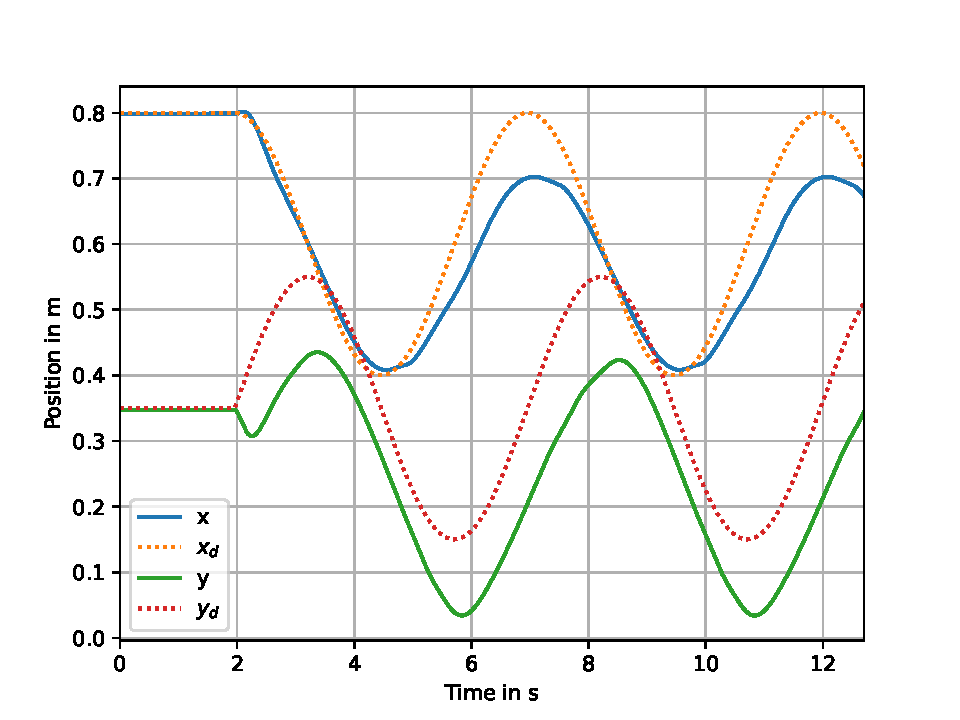
\includegraphics[width=\textwidth]{SRC/CircleTraj_small_kp_x_x_d.pdf} % Replace with your image
        \caption{$x$ and $x_d$ plotted over two revolutions.}
        \label{fig:SmallKpCircXD}
    \end{subfigure}
    \hfill
    % Subfigure 2
    \begin{subfigure}[t]{0.48\textwidth}
        \centering
        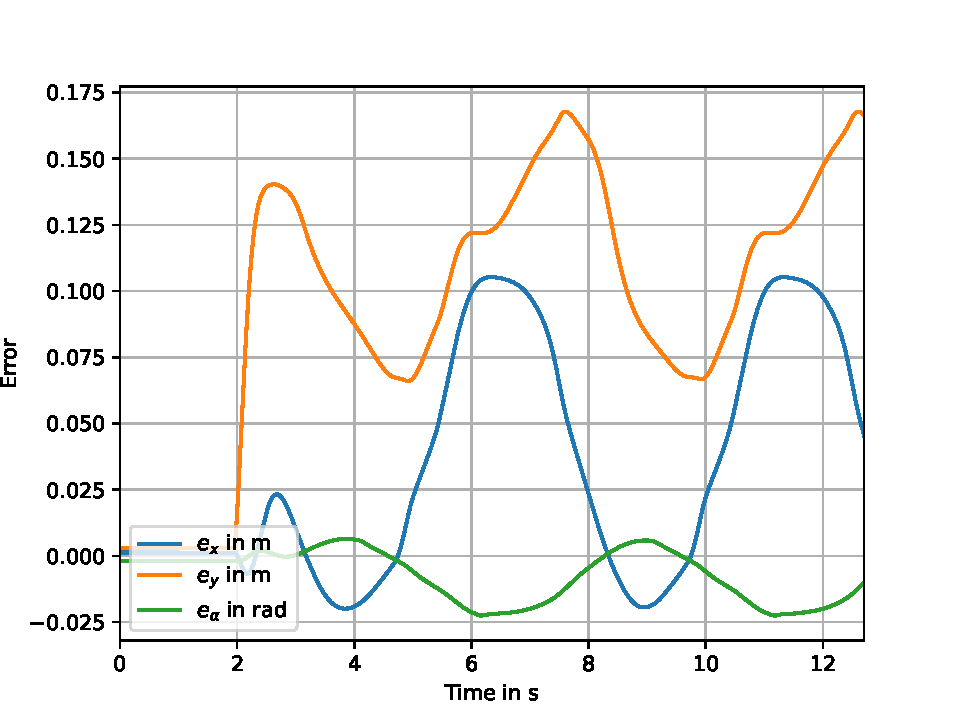
\includegraphics[width=\textwidth]{SRC/CircleTraj_small_kp_exeyea.pdf} % Replace with your image
        \caption{$e_x$, $e_y$ and $e_\alpha$ plotted over two revolutions.}
        \label{fig:SmallKpCircEX}
    \end{subfigure}
    
    \caption{Proj2 control with smaller gains: $k_{p1}$=800, $k_{p2}$=600, $k_{p2}$=200, $k_{v1}$=40, $k_{v2}$=40, $k_{v3}$=40.}
    \label{fig:SmallKpCirc}
\end{figure}

\begin{figure}[H]
    \centering
    % Subfigure 1
    \begin{subfigure}[t]{0.48\textwidth}
        \centering
        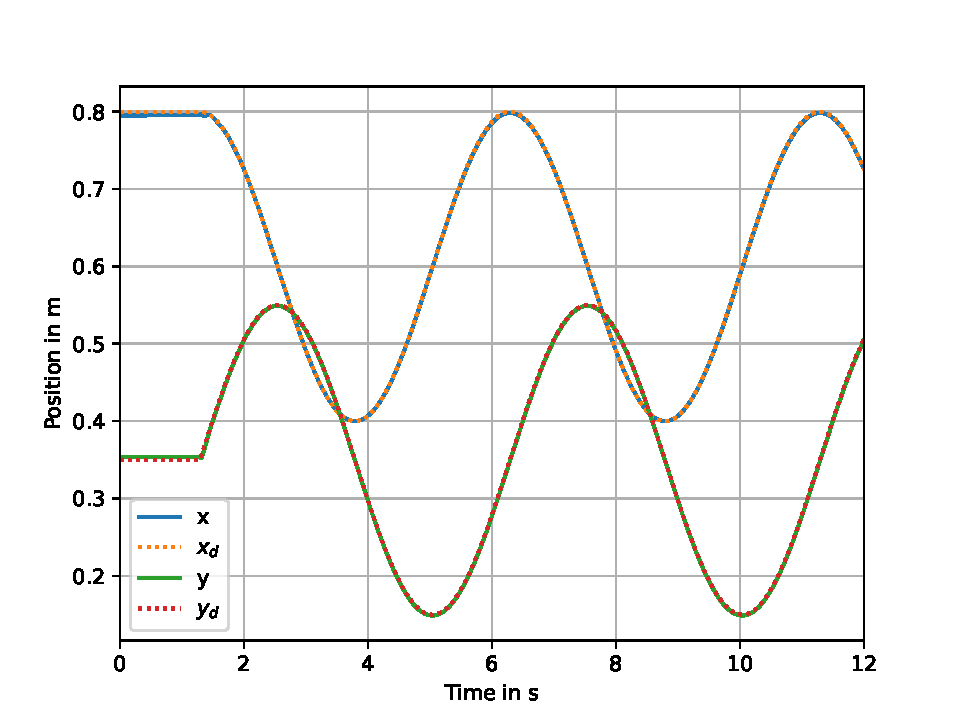
\includegraphics[width=\textwidth]{SRC/CircleTraj_large_kp_x_x_d.pdf} % Replace with your image
        \caption{$x$ and $x_d$ plotted over two revolutions.}
        \label{fig:LargeKpCircXD}
    \end{subfigure}
    \hfill
    % Subfigure 2
    \begin{subfigure}[t]{0.48\textwidth}
        \centering
        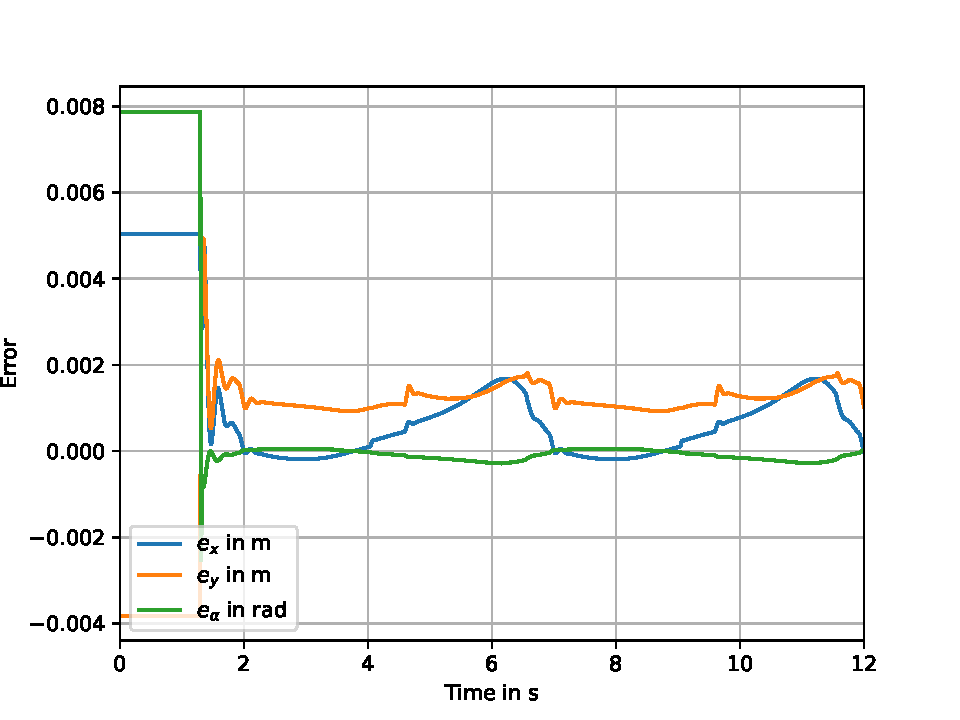
\includegraphics[width=\textwidth]{SRC/CircleTraj_large_kp_exeyea.pdf} % Replace with your image
        \caption{$e_x$, $e_y$ and $e_\alpha$ plotted over two revolutions.}
        \label{fig:LargeKpCircEX}
    \end{subfigure}
    
    \caption{Proj2 control with higher gains: $k_{p1}$=99400, $k_{p2}$=65400, $k_{p2}$=33400, $k_{v1}$=1240, $k_{v2}$=1240, $k_{v3}$=140.}
    \label{fig:LargeKpCirc}
\end{figure}



\begin{figure}[H]
    \centering
    % Subfigure 1
    \begin{subfigure}[t]{0.48\textwidth}
        \centering
        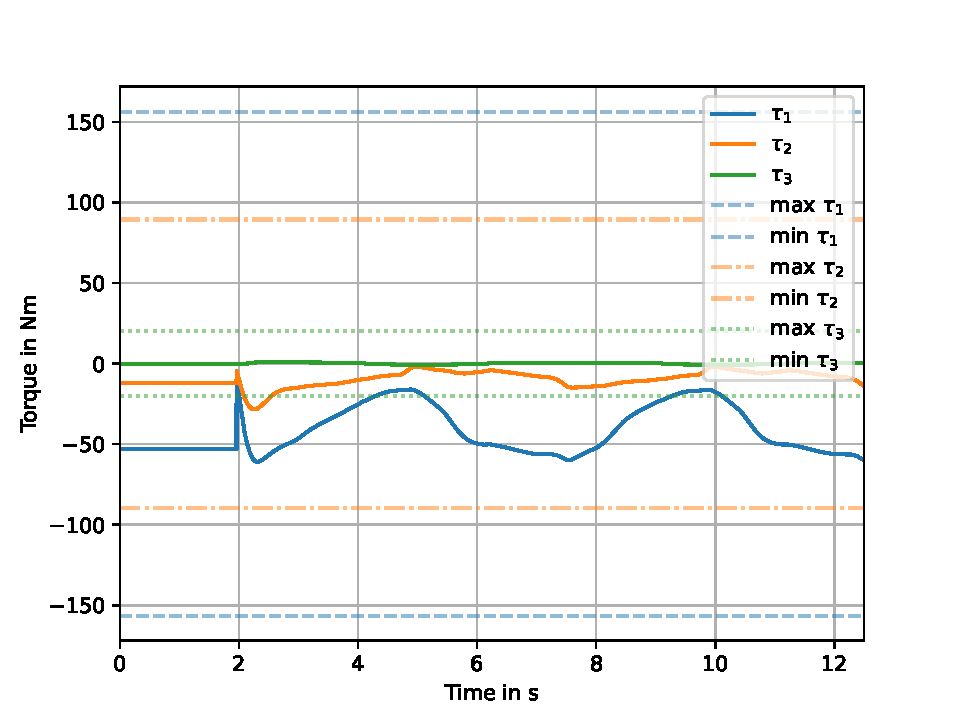
\includegraphics[width=\textwidth]{SRC/CircleTraj_small_kp_tau.pdf} % Replace with your image
        \caption{$\tau$ for gains: $k_{p1}$=800, $k_{p2}$=600, $k_{p2}$=200, $k_{v1}$=40, $k_{v2}$=40, $k_{v3}$=40.}
        \label{fig:HighTau}
    \end{subfigure}
    \hfill
    % Subfigure 2
    \begin{subfigure}[t]{0.48\textwidth}
        \centering
        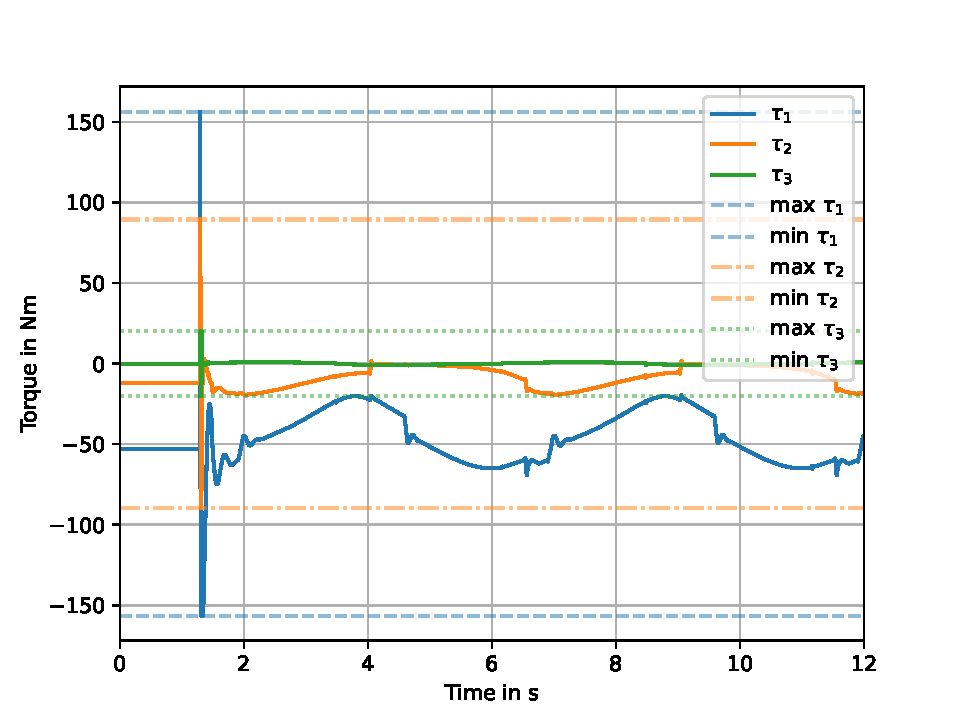
\includegraphics[width=\textwidth]{SRC/CircleTraj_large_kp_tau.pdf} % Replace with your image
        \caption{$\tau$ for gains: $k_{p1}$=99400, $k_{p2}$=65400, $k_{p2}$=33400, $k_{v1}$=1240, $k_{v2}$=1240, $k_{v3}$=140.}
        \label{fig:LowTau}
    \end{subfigure}
    \caption{Proj2 control $\tau$ for lower and higher gainset.}
    \label{fig:TauComparison}
\end{figure}









\subsection{Project3-Parabolic Blend} 
%First, we have to compute $ t_{f,min}$. We need this later for calculing the blend time $t_b$.\\
%The minimum parabolic blend trajectory consist of 2 blend phases. then $tf_{min} = 2 \cdot tb $
%The end effector has to make 3 full circles then,  $\beta(t_{f,min}) = 6 \pi$\\
%After one blend phase we have $\beta(t_b) = 0.5 \cdot \Ddot{\beta}_{max} \cdot t_b^2$. \\
%After two blend phases (complete trajectory) we have $\beta(t_{f,min}) = \Ddot{\beta}_{max} \cdot t_b^2 $ \\
%Now we can write $\Ddot{\beta}_{max}  \cdot \frac{t_{f,min}^2}{4} =  6 \cdot \pi$ \\
%Now we have $t_{f,min}^2 = \frac{24 \cdot \pi }{\Ddot{\beta}_{max}} = 300$, with $ \Ddot{\beta}_{max} = \frac{2 \pi}{25} $ \\
%then, \\ $ t_{f, min} =17.32 s$

First, we have to compute \( t_{f,min} \). We need this later for calculating the blend time \( t_b \). \\
The minimum parabolic blend trajectory consists of two blend phases. Then, \( t_{f,min} = 2 \cdot t_b \). \\
The end effector has to make 3 full circles, so \( \beta(t_{f,min}) = 6 \pi \). \\
After one blend phase, we have \( \beta(t_b) = 0.5 \cdot \Ddot{\beta}_{max} \cdot t_b^2 \). \\
After two blend phases (complete trajectory), we have \( \beta(t_{f,min}) = \Ddot{\beta}_{max} \cdot t_b^2 \). \\
Now we can write:
\[
\Ddot{\beta}_{max} \cdot t_b^2 = 6 \pi
\]
So, solving for \( t_b^2 \), we get:
\[
t_b^2 = \frac{6 \pi}{\Ddot{\beta}_{max}}.
\]
Now we can substitute this into the expression for \( t_{f,min}^2 \):
\[
t_{f,min}^2 = 4 \cdot t_b^2 = 4 \cdot \frac{6 \pi}{\Ddot{\beta}_{max}} = \frac{24 \pi}{\Ddot{\beta}_{max}}.
\]
Substituting \( \Ddot{\beta}_{max} = \frac{2 \pi}{25} \), we get:
\[
t_{f,min}^2 = \frac{24 \pi}{\frac{2 \pi}{25}} = 24 \pi \cdot \frac{25}{2 \pi} = 300.
\]
Thus, we find:
\[
t_{f,min} = \sqrt{300} \approx 17.32 s.
\]
We chose $t_{f}= 20s$ \\\\\\
2-Trajectory equations \\ \\

\textbf{1. Acceleration phase:}  for \( t \in [0, t_b] \)
\[
\beta(t) =  \frac{1}{2} \cdot \Ddot{\beta}_{max} \cdot t^2
\]

\textbf{2. Constant velocity phase:} for \( t \in [t_b, t_b + t_c] \)
\[
\beta(t) = \frac{1}{2} \Ddot{\beta}_{max} t_b^2 + \dot{\beta}_{\text{max}} (t - t_b) \quad with \quad \dot{\beta}_{\text{max}} = t_b \cdot \Ddot{\beta}_{max} 
\]


\textbf{3. Deceleration phase:}  for \( t \in [t_b + t_c, t_f] \)
\[
\beta(t) = \beta(t_f) - \frac{1}{2} \Ddot{\beta}_{max} (t - t_f)^2
\]
As we see to get the trajectory we have to find $t_b$: \\
\[
\beta(t_b) =0.5 \Ddot{\beta}_{max} t_b^2
\]
\[
\beta(t_c) =0.5 \Ddot{\beta}_{max} t_b^2 + \Ddot{\beta}_{max} t_b (t_c-t_b) 
\]
\[
\beta(t_c) =0.5 \Ddot{\beta}_{max} t_b^2 + \Ddot{\beta}_{max} t_b (t_f-2t_b) 
\]
\[
\beta(t_c) =-1.5 \Ddot{\beta}_{max} t_b^2 + t_b \cdot t_f 
\]
\[
\beta(t_f) =\beta(t_c) + \beta(t_b) = 0.5 \Ddot{\beta}_{max} t_b^2  -1.5 \Ddot{\beta}_{max} t_b^2 + \Ddot{\beta}_{max} t_b \cdot t_f = 6 \pi
\]
\[
\beta(t_f) = -\Ddot{\beta}_{max} t_b^2 + \Ddot{\beta}_{max} t_b \cdot t_f = 6 \pi
\]
\[
 \Ddot{\beta}_{max} t_b^2 - \Ddot{\beta}_{max} t_b \cdot t_f +6 \pi = 0
\]
\[
t_b =  \frac{t_f \pm \sqrt{ t_f^2- \frac{6\pi}{\Ddot{\beta}_{max} }}}{2}
\]

We chose $\Ddot{\beta}_{max} = \frac{2 \pi}{25s^2} \quad and \quad t_f = 20s $\\
So we get $t_{b1}= 5 s \quad and\quad t_{b2} =15s $ \\
we have $ t_f-2t_{b2} = -10s$ this must be within the time interval of the trajectory. Also we reject this solution.  
and the solution is $t_{b1}=t_b=5s$. \\
Now we have  equation of the angular position of the end effort but we need for the simulation a coordinate.  
\[
 x=r cos(\beta(t))+x_0 
\]
\[
 y=r sin(\beta(t))+y_0
\]
\[
 \dot{x}=-r\dot{\beta}(t)sin(\beta(t))
\]
\[
\dot{y}=r\dot{\beta}(t)cos(\beta(t)) 
\]

\begin{figure}[H]
    \centering
    % Subfigure 1
    \begin{subfigure}[t]{0.48\textwidth}
        \centering
        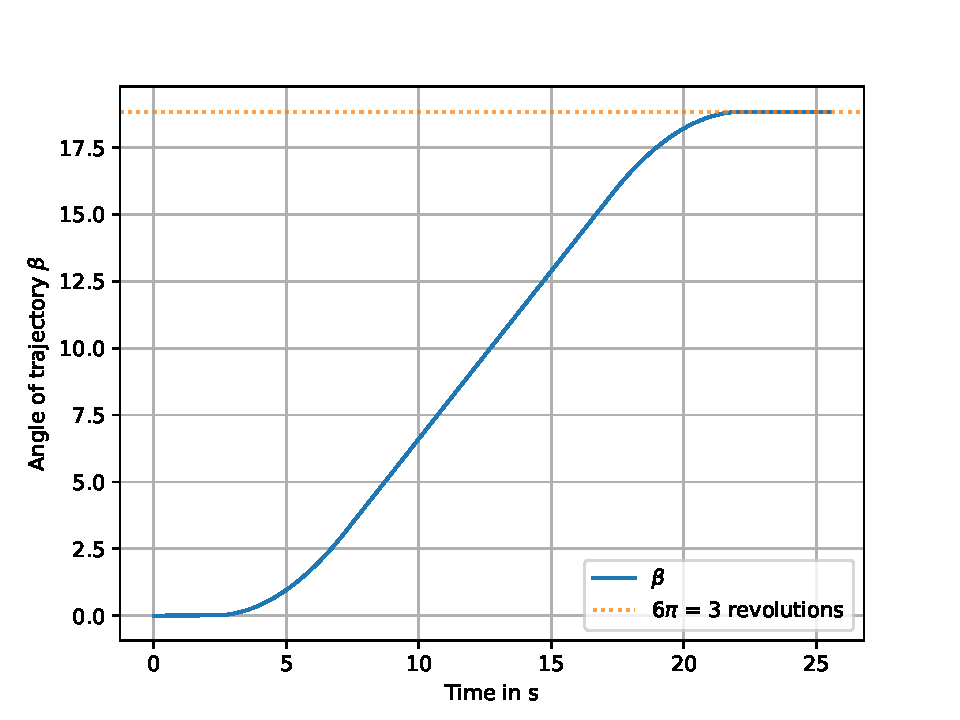
\includegraphics[width=\textwidth]{SRC/Proj3Beta.pdf} % Replace with your image
        \caption{Position of angle $\beta$(t).}
        \label{fig:angular_position}
    \end{subfigure}
    \hfill
    % Subfigure 2
    \begin{subfigure}[t]{0.48\textwidth}
        \centering
        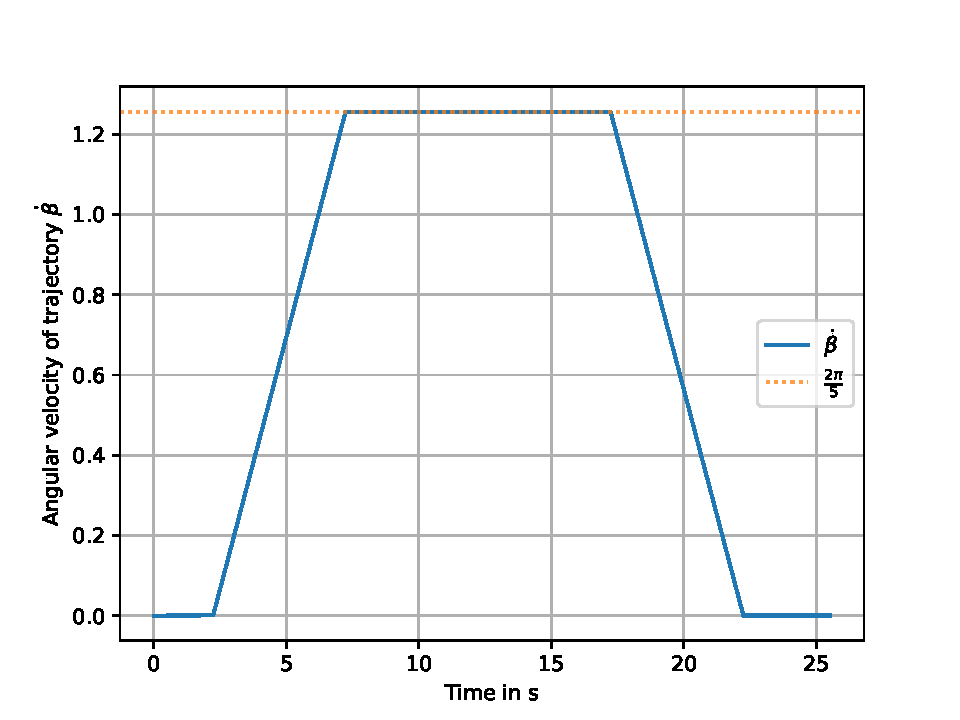
\includegraphics[width=\textwidth]{SRC/Proj3BetaDot.pdf} % Replace with your image
        \caption{Angular velocity $\dot{\beta}(t)$.}
        \label{fig:angular velocity}
    \end{subfigure}

  \caption{Position and angular velocity in proj3.}
    \label{fig:TauComparison}
\end{figure}


While choosing the same gains as in the proj2 control we can see that through the parabolic blends we do not required rapid movements in the beginning of the motion and therefore experience no spike in torque at the start of the motion (see Figure \ref{fig:Proj3_tau}). As we can additionally see in Figure \ref{fig:Xd_yD_Proje3} the desired trajectory is followed well. So in theory this enables us to use higher gains to have less error while still fulfilling the constraints on maximum torque expense. 

\begin{figure}[H]
    \centering
    % Subfigure 1
    \begin{subfigure}[t]{0.48\textwidth}
        \centering
        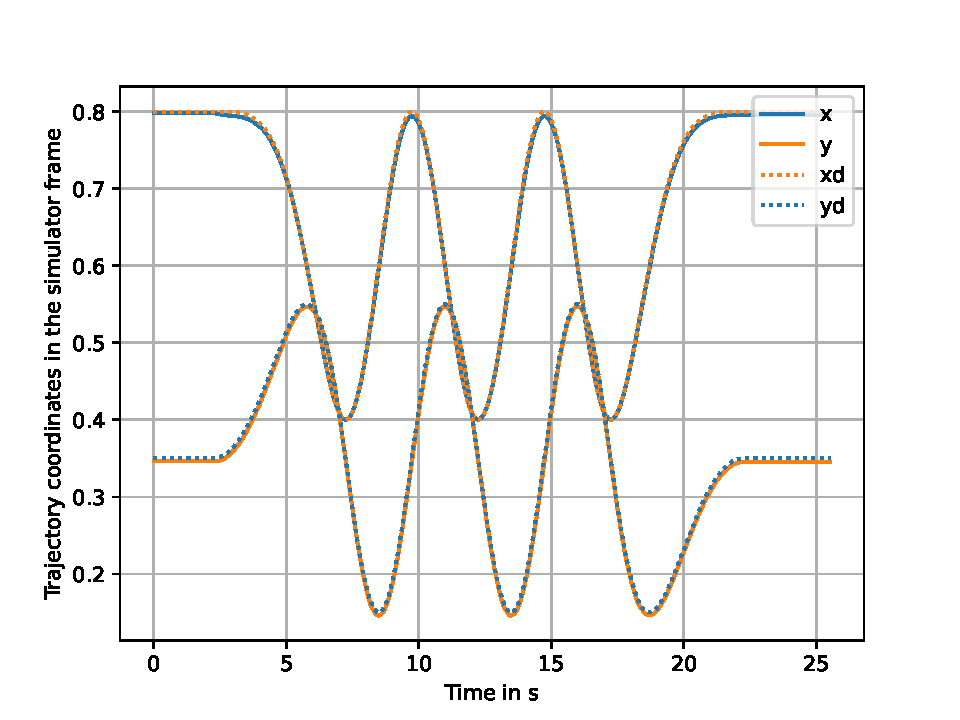
\includegraphics[width=\textwidth]{SRC/Proj3X_Xd_y_yd.pdf} % Replace with your image
        \caption{Desired trajectory xd/yd and controlled trajectory x/y.}
        \label{fig:Xd_yD_Proje3}
    \end{subfigure}
    \hfill
    % Subfigure 2
    \begin{subfigure}[t]{0.48\textwidth}
        \centering
        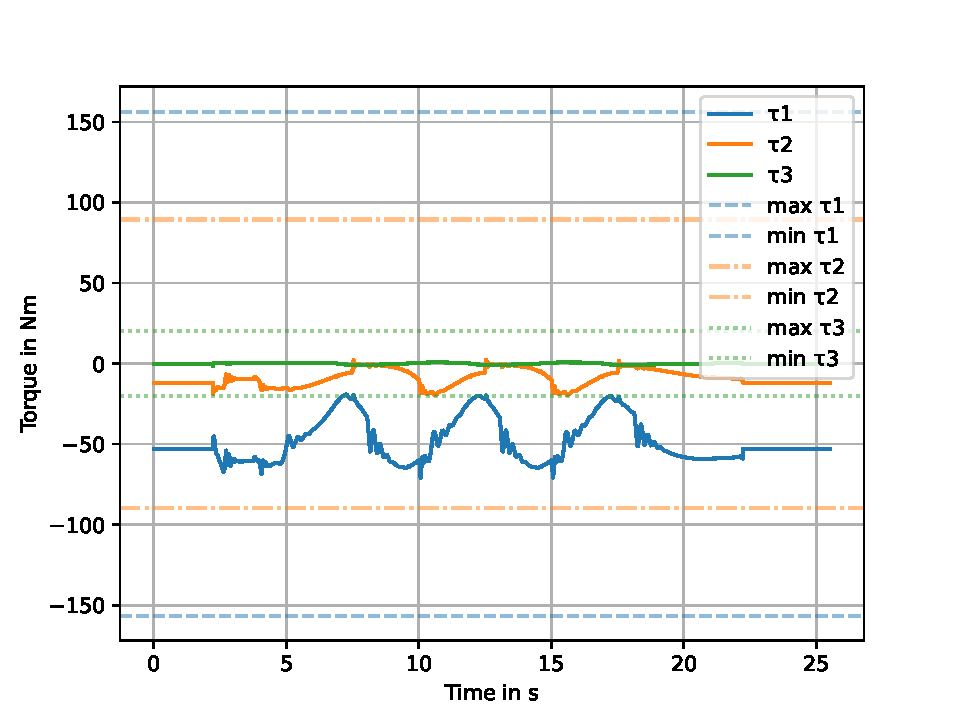
\includegraphics[width=\textwidth]{SRC/Proj3Tau.pdf} % Replace with your image
        \caption{Torque required for trajectory tracking.}
        \label{fig:Proj3_tau}
    \end{subfigure}

  \caption{Further graphs displaying trajectory and torque.}
    \label{fig:Proj3_tau_xd}
\end{figure}


\begin{table}[h]
    \centering
    \begin{tabular}{ |p{3cm}|p{0.5cm}|p{0.5cm}|p{0.5cm}|p{0.5cm}|p{0.5cm}|p{0.5cm}|p{0.5cm}|p{0.5cm}|p{0.5cm}|p{0.5cm}|p{0.5cm}|p{0.5cm}|p{2.5cm}|  } 
        \hline
       Student Name  & A1 & A2 &A3 & A4&A5&B1&B2&C1&C2&C3&C4&C5&Documentation\\
        \hline
       Maxim Fenko  & X & X &X & X& X & X & X & X &X&X&X&X&X\\
        \hline
       Abdelkarim Ben Salah  & X & X & X& X& X& X& X&X & X&X&X&X&X\\
        \hline
        Bryan Oppong-Boateng  & X& X& X& X & X&X &X & &&&&&X\\
        \hline
    \end{tabular}
    \label{Table:MotorSignals}
\end{table}

